%!TeX root = ./../MusterAbschlussarbeit.tex

%##########################################################
% Inhalt
%##########################################################

\clearpage
\chapter{Präsentation der Ergebnisse}

Um den Lernprozess evaluieren zu können, wurden verschiedene Experimente durchgeführt. Diese Experimente werden in diesem Kapitel vorgestellt und ausgewertet.

\section{Agent ohne Spielreglementierung}

Im ersten Schritt überprüfte ich, ob der Agent die Spielregeln selbstständig über Belohnungen erlernen kann. In diesem Versuch sollte der Agent Felder via Index auswählen.
Jedes Kästchen im Spielfeld besaß einen Index zwischen 0-104. Je nach Höhe der gewürfelten Zahl, wurden ebenso viele Feldindizes überprüft. In \ref{tab:Aufbau Actionbuffer Versuch 1} ist der Aufbau des Actionbuffers dargestellt. 

\begin{table}[!h]
    \centering
    \begin{tabular}{|c|c|c|c|}
    \hline
    \textbf{Index} & \textbf{Bezeichnung} & \textbf{Datentyp} & \textbf{Wertebereich} \\
    \hline
    1 & Index des zu wählenden Farbwürfels & int & 0-1 \\
    \hline
    2 & Index des zu wählenden Zahlenwürfels & int & 0-1 \\
    \hline
    3 & Feldindex & int & 0-104 \\
    \hline
    4 & Feldindex & int & 0-104 \\
    \hline
    5 & Feldindex & int & 0-104 \\
    \hline
    6 & Feldindex & int & 0-104 \\
    \hline
    7 & Feldindex & int & 0-104 \\
    \hline
    \end{tabular}
    \caption{Aufbau Actionbuffer}
    \label{tab:Anpassung Actionbuffer Versuch Agent ohne Spielimplementierung}
\end{table}

Nach der Auswahl aller potenziell abzukreuzenden Feldern wurde überprüft, ob der Zug legal ist. Die Überprüfung belief sich auf folgende Kriterien: Mindestens ein Feld musste verfügbar sein, alle Felder mussten benachbart und der selben Farbe sein. Illegale Züge zogen negative Rewards mit sich, legal ausgeführte Züge dagegen positive. \\
Diese Herangehensweise führte nicht zum gewünschten Ergebnis. Auch nach einigen Stunden des Trainings, konnte der Agent nur sehr selten legale Züge durchführen. Dem Agent war es nicht möglich in der begrenzten Trainignszeit den Zusammenhang der Beobachtungen zu den gegebenen Rewards festzustellen.
Dennoch ist der Ansatz nicht gänzlich falsch. Mit einem hohen Rechenaufwand, könnte der Agent auch die Spielregeln erlernen, es würde nur sehr viel Zeit kosten. 




\newpage
\section{Agent mit zusätzlichen Belohnungen}
In diesem Versuch bekam der Agent zusätzlich zu den ursprünglichen Rewards, zusätzliche Belohnungen für bestimmte Aktionen. Diese Belohnungen sollten den Agenten zu komplexeren Spielzielen leiten, um so schneller zu einer optimalen Policy zu gelangen.
In ref{tab:rewards2} sind alle zusätzlichen Rewards ersichtlich. Der Versuch wurde 2.4Mio Spielzüge ausgeführt. Dieser Zeitraum ist, wie sich im Verlauf der folgenden Experimente herrausstellt, relativ kurz. Da sich jedoch ein negatives Ergebnis abzeichnete, wurde auf längeres Training verzichtet.  

\begin{table}[!htbp]
    \centering
    \begin{tabular}{|c|c|}
    \hline
    \textbf{Aktion} & \textbf{Erhaltene Belohnung} \\
    \hline
    Abkreuzen von Feldern & 0.02f pro Feld \\
    \hline
    Abkreuzen eines gesamten Clusters & 0.04f pro Feld \\
    \hline
    Wahl eines Würfelpaars ohne legale Züge & -50.0f \\
    \hline
    Wahl eines Jokers ohne verfügbare Joker & -50.0f \\
    \hline
    \end{tabular}
    \caption{Zusatzbelohnungen für verschiedene Aktionen}
    \label{tab:rewards2}
\end{table}



Die  Grafiken \ref{fig:average_points} und \ref{fig:average_rewards} zeigen deutlich, dass je länger das Training voranschritt, die durchschnittlich erreichten Punkte pro Spiel sanken.
Die zusätzlichen Belohnungen führten dazu, dass der Agent nicht versuchte Spalten abzukreuzen oder Farben komplett auszufüllen, da er das Abkreuzen von Clustern für deutlich effizienter hielt, um seine Belohnungen zu maximieren.
Obwohl die Belohnungen für erreichte Spalten oder komplett ausgefüllte Farben mehr Punkte ergaben. 

\begin{figure}[!h]
    \centering
    \includegraphics[scale=0.6]{Bilder/average_points.png}
    \caption{Durchschnittliche Punkte des Agenten mit Zusatzbelohnungen}
    \label{fig:average_points}
\end{figure}

\begin{figure}[!h]
    \centering
    \includegraphics[scale=0.6]{Bilder/average_rewards.png}
    \caption{Durchschnittliche Belohnungen des Agenten mit Zusatzbelohnungen }
    \label{fig:average_rewards}
\end{figure}

\section{Vergleich trainiert und untrainiert}
In diesem Experiment, werden die erreichten Punkte und Rewards eines untrainierten Agenten gegenüber den erzielten Ergebnissen eines trainierten Agenten gestellt. Der trainierte Agent hat bereichts 25 Mio. Spielzüge absolviert, was ungefähr 830k gespielten Spielen entspricht.
Der untrainierte Agent trainiert ein neu initialisiertes NN, welches zufällig gewählte Kantengewichte zwischen den Neuronen erhält.
Wie an den Grafiken \ref{fig:untrained_rewards} und \ref{fig:untrained_points} zu erkennen ist, hat der trainierte Agent tatsächlich einen höheren Durchschnitt an erzielten Punkten pro Spiel. Auch die gesammlten Rewards sind bei dem trainierten Agenten höher.
Dies liegt daran, dass die Rewards so festgelegt sind, dass der Agent sie nur erhält, wenn er auch im Spiel punktet.
Schon während des Trainings war ein merklicher Unterschied festzustellen, deshalb war das Ergebnis dieses Experiments zu erwarten.


\begin{figure}[!h]
    \centering
    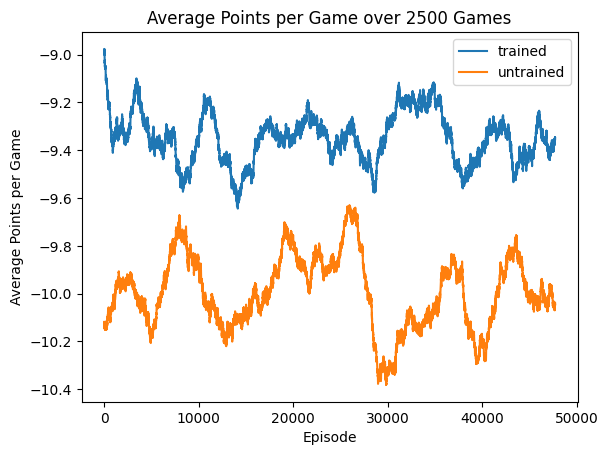
\includegraphics[scale=0.6]{Bilder/points_trained_vs_untrained.png}
    \caption{Durchschnitt der erreichten Punkte pro Spiel }
    \label{fig:untrained_points}
\end{figure}
\begin{figure}[!h]
    \centering
    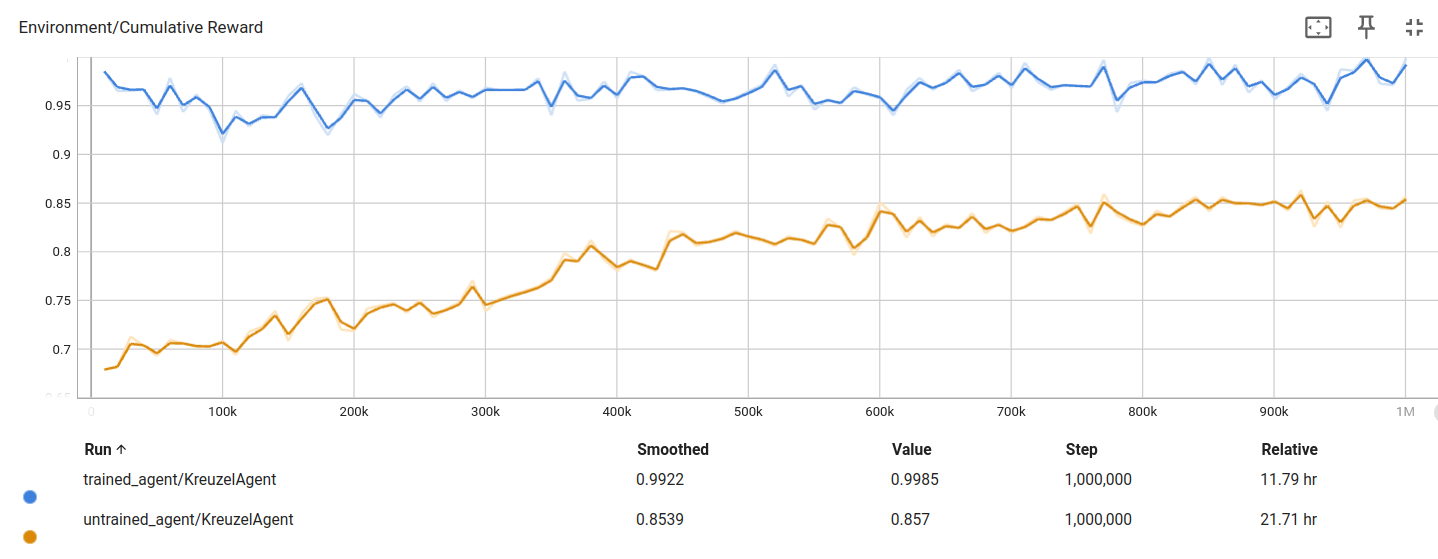
\includegraphics[scale=0.3]{Bilder/rewards_untrained.png}
    \caption{Übersicht der gesammelten Belohnungen}
    \label{fig:untrained_rewards}
\end{figure}

\newpage
\section{Training auf Sonderfeldern}
In diesem Experiment wurden die erreichten Puntke und Rewards des trainierten Agenten gegen einen Agenten, welcher mit Sonderfeldern trainiert wurde verglichen. Beide Agenten wurden mit dem selben vortrainierten Modell instanziiert. \ref{fig:specialFields} stellt den Aufbau der Trainingsumgebunng dar. Dieser Versuch sollte überprüfen, ob ein Agent im Verlauf besser erlernen kann kann welche Stellen im Beobachtungsvektorvektor für welche Information zuständig sind. 

\begin{figure}[!h]
    \centering
    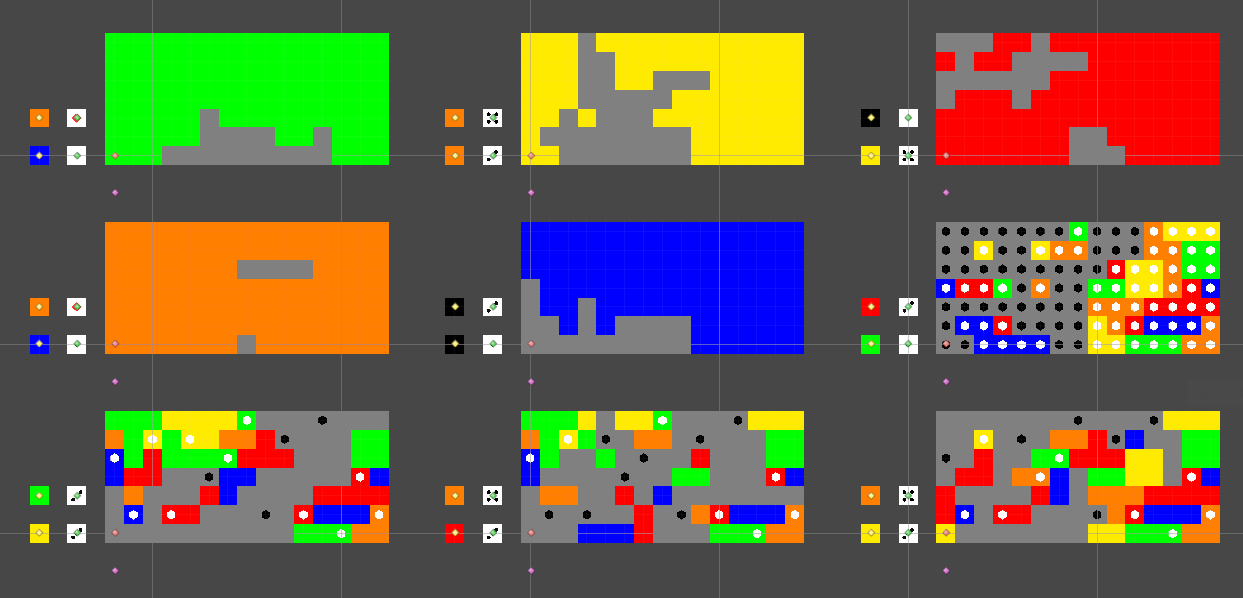
\includegraphics[scale=0.4]{Bilder/specialFields.png}
    \caption{Übersicht der speziellen Felder}
    \label{fig:specialFields}
\end{figure}

In der Grafik \ref{fig:specialFields} ist das Training mit den speziellen Feldern dargestellt. Jedes der Feld hat gewisse Besonderheiten, welche sich zu den normalen Spielfeldern abgrenzen.
Fünf Felder sind in einer kompletten Farbidentität eingefärbt. In \ref{lst:DiceShift} wurde der Zahlenwürfel manipuliert um häufiger die entsprechende Farbe zu werfen. Diese Felder sollten dem Agenten besser den Zusammenhang des Farbwürfels und des gewählten Farbidentität der Kästchen näherbringen.
In dem anderen Spielfeld ist jedes Feld als Sternfeld markiert. Dies sollte dem Agenten zeigen, dass jedes Feld mit markierten Sternen mehr Punkte bringt.
Bei den anderen drei Feldern ist jedes Feld von vorn herein als verfügbar markiert. Dies sollte zum einen das Konzept des verfügbaren Feldes vermitteln, zum anderen dem Agenten ermöglichen das Feld weiter als normal zu explorieren, um die komplexen Ziele des Spiels leichter zu erreichen. \\
Das Training mit speziellen Feldern führte zu einer Verschlechterung des Ergebnisses. \\
Aus der Grafik \ref{fig:special_points} lässt sich ableiten, dass das Modell, welches mit speziellen Feldern trainiert wurde, im Durchschnitt weniger Punkte erhalten erreichte, als der normal trainierte Agent. Dieses Training führte nicht zu einer Verbesserung des Modells. Ursache hierfür liegt sicher im Spielfeld, in welchem alle Felder als Sternfelder markiert wurden. Hier konnte der Agent willkürlich Züge ausführen und bekam überdurchschnittlich viele Punkte. Deshalb priorisierte der Agent nicht mehr die eigentlichen Ziele, was wiederum zur Folge hatte, dass die Leistung des Agenten auf dem eigentlichen Feld schlechter wurde. 

\begin{figure}[!h]
    \centering
    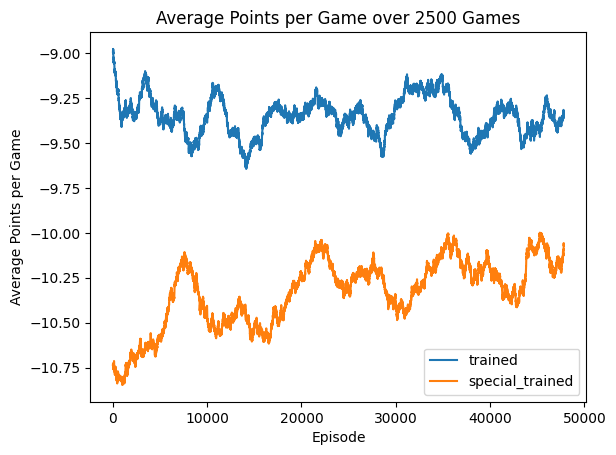
\includegraphics[scale=0.6]{Bilder/points_special_trained.png}
    \caption{Durchschnitt der erreichten Punkte beider Agenten}
    \label{fig:special_points}
\end{figure}

 \newpage
\section{Training mit mehr Spielzügen}

In diesem Experiment trainierte der Agent mit mehr zur Verfügung stehenden Spielzügen. Dadurch konnte der Agent das Feld besser explorieren und insgesamt mehr Aktionen auslösen welche zu Belohnungen führten. Dies hat zur Folge, dass auch schwierig erreichbare Rewards ausgelöst wurden, welche somit vom Agent erlernt werden konnten. 
Die Grafik \ref{fig:turns_points} zeigt, dass das Experiment eine Verbesserung des Models zur Folge hatte, da im Durchschnitt etwas mehr Punkte erreicht wurden.

\begin{figure}[!h]
    \centering
    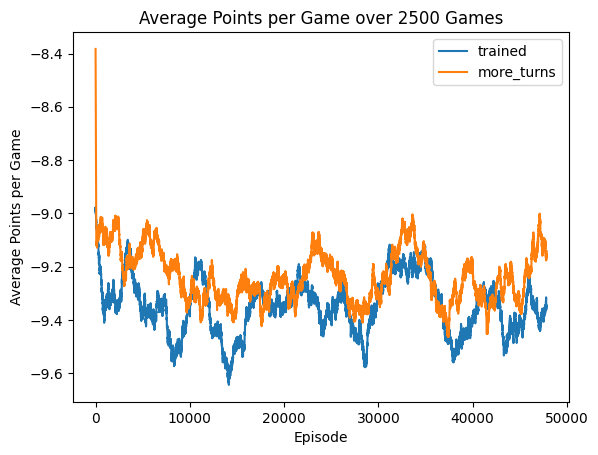
\includegraphics[scale=0.6]{Bilder/points_more_turns.png}
    \caption{Vergleich 'Mehr Züge' und 'trainierter Agent'}
    \label{fig:turns_points}

\end{figure}

\newpage
\section{Überprüfung auf Überanpassung}
In diesem Experiment sollte der Agent auf Überanpassung überprüft werden. Trainierter und untrainierter Agent spielten das Spiel nach normalen Spielregeln auf einem anderen Spielfeld.
In den Grafiken \ref{fig:orange_points} und \ref{fig:orange_rewards} ist erkennbar, dass beide Agenten ungefähr die selben Rewards gesammelten haben. Der untrainierte Agent konnte im Durchschnitt jedoch etwas mehr Punkte sammeln.
Dies schließt darauf, dass der Agent tatsächlich nur auf dem im Training verwendeten Spielfeld gut performen kann und neue Spielfelder erst erlernen muss.
Interessant ist weiterhin, dass der Durchschnitt aller Punkte etwa 2 Punkte über dem des anderen Spielfeldes liegt, was auf eine höhere Schwierigkeit des schwarzen Spielfeldes hinweist.


\begin{figure}[!h]
    \centering
    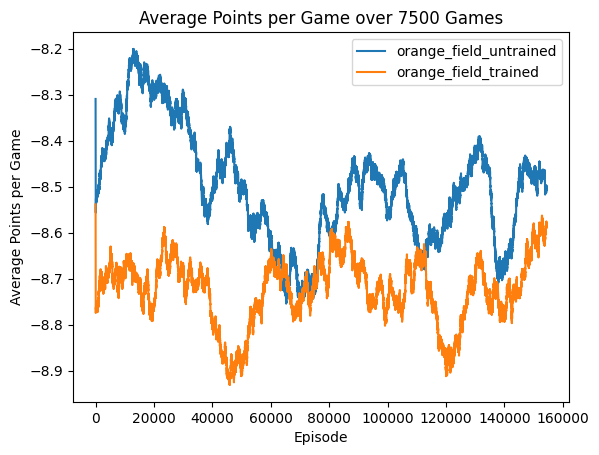
\includegraphics[scale=0.6]{Bilder/points_orange_field.png}
    \caption{Vergleich Punkte 'trainiert' und 'untrainiert' auf orangen Spielfeld}
    \label{fig:orange_points}
\end{figure}
\begin{figure}[!h]
    \centering
    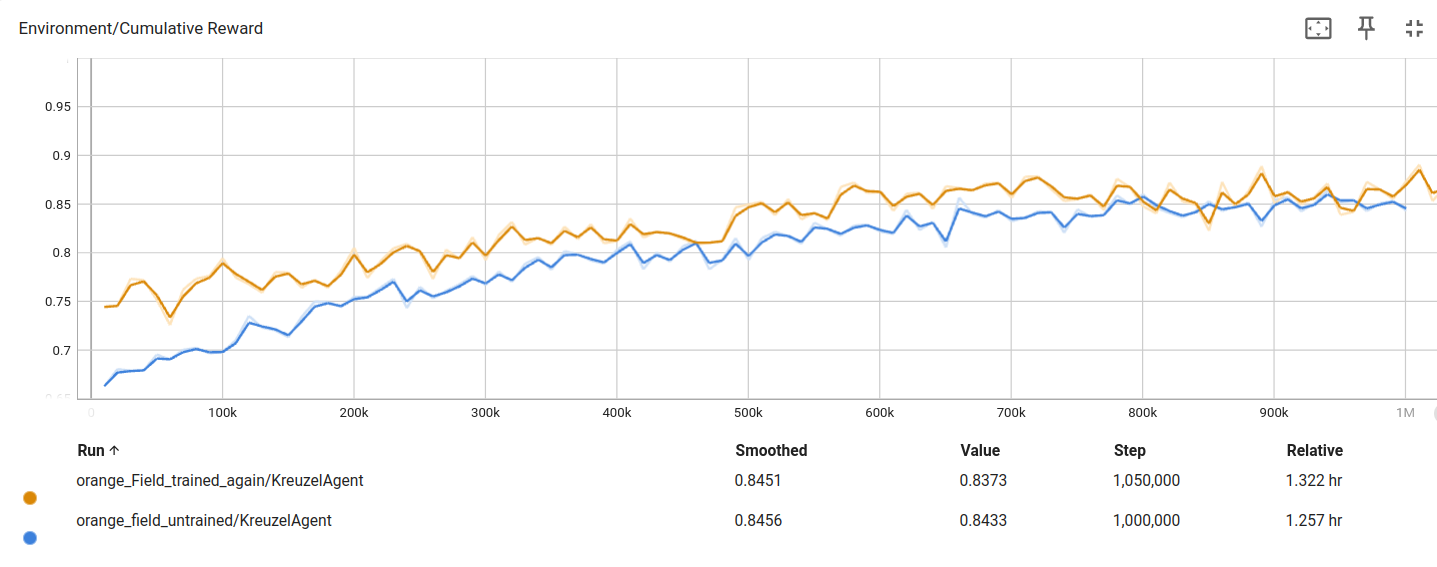
\includegraphics[scale=0.3]{Bilder/rewards_orange_field.png}
    \caption{Übersicht gesammelte Rewards auf orangen Spielfeld}
    \label{fig:orange_rewards}

\end{figure}

\newpage
\section{Training auf Minifeld}
Um zu überprüfen, ob ein kleineres Feld  einen positiven Effekt auf das Training hat, habe ich bei einem Spielfeld 3 Zeilen abgeschnitten und ließ einen Agenten darauf trainieren. \ref{fig:miniFeld} zeigt die Lernumgebung für dieses Experiment für einen Agenten.
Im Anschluss überprüfte ich die Leistung des Agenten auf dem normalen Spielfeld gegenüber einem untrainierten Agenten. Da die Observations von Modellen gleich bleiben müssen, entscheid ich mich nicht mehr vorhandene Kästchen mit Nullen im Vektor zu präsentieren. \ref{lst:PushEmptyField} zeigt den Quellcode zum übergeben eines leeren Feldes.

\lstinputlisting[language=csh, label={lst:PushEmptyField}, caption={Befüllen des Beobachtungsvektor mit leerem Feld}]{Programmcode/PushEmptyField.cs}

Die Grafiken \ref{fig:Minifeld_rewards} und \ref{fig:Minifeld_points} zeigen den Durchschnitt der erreichten Punkte pro Spiel und die gesammelten Blohnungen während des Trainings.
Es wird ersichtlich, dass der mit einem kleinen Feld vortrainierte Agent schlechter performt, als die beiden anderen. Belohnungen wurden auch hier nur verteilt, wenn es zur Punktewertung kommt. Deshalb ist es interessant, dass der untrainierte Agent mehr Punkte erreicht, als der auf dem kleinen Feld vortrainierte Agent, obwohl dieser wiederum einen höheren Durchschnitt an Belohnungen erhält. Ursache für das schlechtere Ergebnis, ist auf die Überanpassung zurückzuführen. So wurde beim Training auf dem kleinen Feld ausschließlich dieses Feld erlernt und nicht eine gute Spielweise. 


\begin{figure}[!h]
    \centering
    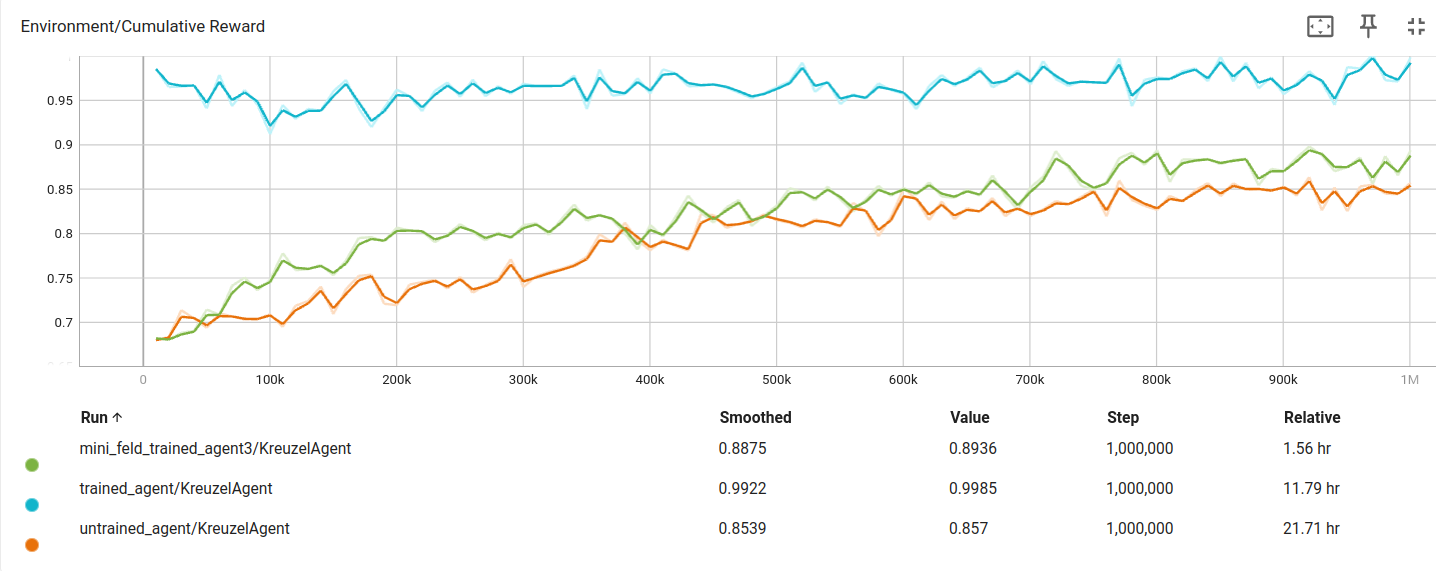
\includegraphics[scale=0.3]{Bilder/rewards_minifield.png}
    \caption{Gesammelte Belohnungen mit Minifeld}
    \label{fig:Minifeld_rewards}
\end{figure}

\begin{figure}[!h]
    \centering
    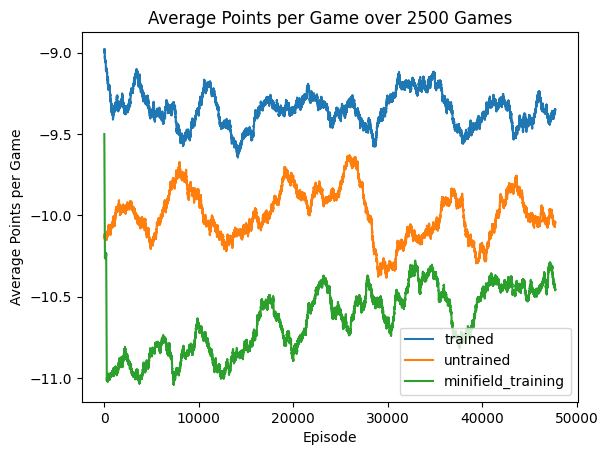
\includegraphics[scale=0.5]{Bilder/points_minifeld.png}
    \caption{Vergleich erreichte Punkte}
    \label{fig:Minifeld_points}
\end{figure}


\section{Training blinder Agent}
In diesem Experiment bekam der Agent lediglich die Würfel, die Anzahl der verbleibenden Joker und die aktuelle Runde des Spiels übergeben.
Dieser Versuch sollte überprüfen, wie gut ein Agent, der die aktuelle Informationen vom  Spielfeld nicht erhält, perfomt. Dies sollte überprüfen, ob das trainierte Modell tatsächlich besser ist, als eine rein zufällige Spielweise.
Da die Auswahl der Felder durch  zufällige Interpolation aller möglichen Felder abläuft, kann der blinde Agent normal spielen. Durch den Versuchsaufbau veringert sich der Beobachtungsvektor von 916 auf eine Größe von 15 Informationen. Dies führte dazu, dass der Agent schnell zu seiner optimalen Policy gelangen konnte. Auch wenn der Agent das Spielfeld nicht sieht, kann er dieses implizit erlernen. Dieser Prozess wäre allerdings nicht sonderlich robust, wäre sehr lernintensiv und würde nicht auf anderen Feldern funktionieren. Der Agent konnte bereits nach sehr kurzer Zeit von etwa 400k Lernschritten gegen sein Maximum konvergieren, wie in \ref{fig:onlydice_rewards} ersichtlich ist. Dort schneiden sich die beiden grünen Graphen und verbleiben auf ungefähr dem selben Niveau. Dieses Modell wurde insgesamt 5 Mio. Episoden trainiert. Der trainierte Agent konnte sich dagegen kontinuierlich minimal verbessern und erreichte auch nach 25Mio Lernschritten noch keinen Maximalwert. \\
Abbildung \ref{fig:onlydice_points} zeigt, dass auch der blinde Agent im Durchschnitt weniger Punkte erreichen konnte. Dies beweist, dass das Training, trotz der geringen erreichten Punkte, positiv verlaufen ist.


\begin{figure}[!h]
    \centering
    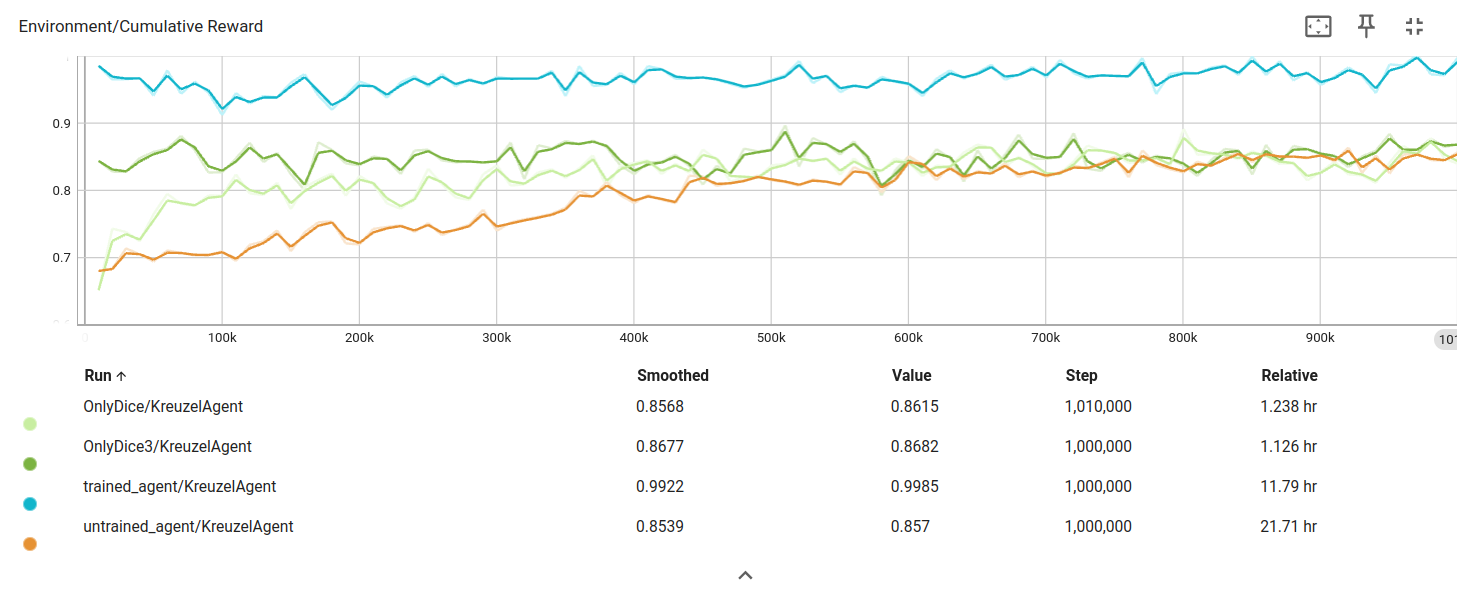
\includegraphics[scale=0.3]{Bilder/rewards_onlydice.png}
    \caption{Gesammelte Belohnungen blinder Agent}
    \label{fig:onlydice_rewards}
\end{figure}

\begin{figure}[!h]
    \centering
    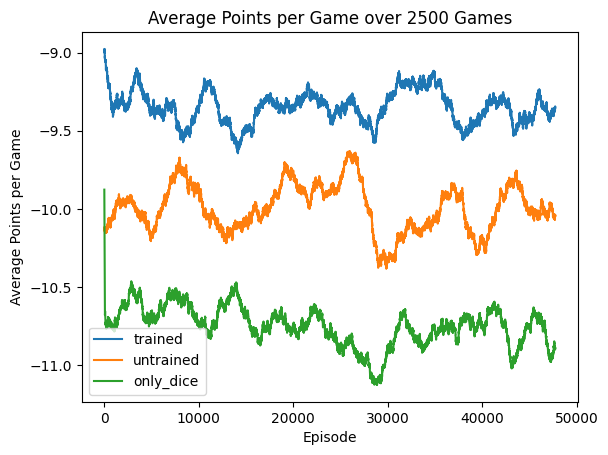
\includegraphics[scale=0.5]{Bilder/points_onlydice.png}
    \caption{Vergleich erreichte Punkte blinder Agent}
    \label{fig:onlydice_points}
\end{figure}